% !TEX root = ../TransportFR.tex


\newcommand{\Blu}[1]{{\color{blue}#1}}
\newcommand{\Red}[1]{{\color{red}#1}}
\newcommand{\iC}{\Red{i}}
\newcommand{\jC}{\Blu{j}}
\newcommand{\aC}{\Red{a}}
\newcommand{\bC}{\Blu{b}}


\ifdefined\otarticle
\newcommand{\myparagraph}[1]{\subsection{#1}}
\else
\newcommand{\myparagraph}[1]{\paragraph{#1}}
\chapter{Le Transport Optimal et ses Applications}
\fi

\label{chap-ot}


%%%%%%%%%%%%%%%%%%%%%%%%%%%%%%%%%%%%%%%%%%%%%%
\section{Le Transport Optimal de Monge}

Gaspard Monge, en plus d'�tre un grand math�maticien, a particip� activement � la r�volution Fran�aise, et a cr�� l'\'Ecole Polytechnique ainsi que l'\'Ecole Normale Sup�rieure. Motiv� par des applications militaires, il a formul� en 1781 le probl�me du transport optimal~\cite{Monge1781}. Il s'est pos� la question du calcul de la fa�on la plus �conomique de transporter de la terre entre deux endroits pour faire des remblais. Dans son texte original, il a fait l'hypoth�se que le co�t du d�placement d'une unit� de masse est �gal � la distance parcourue, mais on peut utiliser n'importe quel co�t adapt� au probl�me � r�soudre. 

%%%%%%%%%%%%%%%%%%%%%%%%%%%%%%%%%%%%%%%%%%%%%%%%%%%%%
\myparagraph{Le probl�me de Monge}

Pour illustrer le probl�me et sa formulation math�matique, int�ressons-nous � la fa�on optimale de distribuer les croissants depuis les boulangeries vers les caf�s, le matin dans Paris. Pour simplifier, nous allons supposer qu'il y a uniquement six boulangeries et caf�s, que l'on peut voir � la figure~\ref{fig:image-cafe} (les boulangeries sont en \Red{rouge} et les caf�s en \Blu{bleu}). Le co�t � minimiser est le temps total des trajets, et l'on note $C_{\iC,\jC}$ le temps entre la boulangerie $\iC \in \{1,\ldots,6\}$  et le caf� $\jC \in \{1,\ldots,6\}$. Par exemple, on a $C_{\Red{3},\Blu{4}}=10$, ce qui signifie qu'il y a dix minutes de trajet entre la boulangerie num�ro $\Red{3}$ et le caf� num�ro $\Blu{4}$. 

\begin{figure}\centering
    \begin{tabular}{@{}c@{\hspace{1mm}}c@{\hspace{4mm}}c@{\hspace{1mm}}c@{}}
        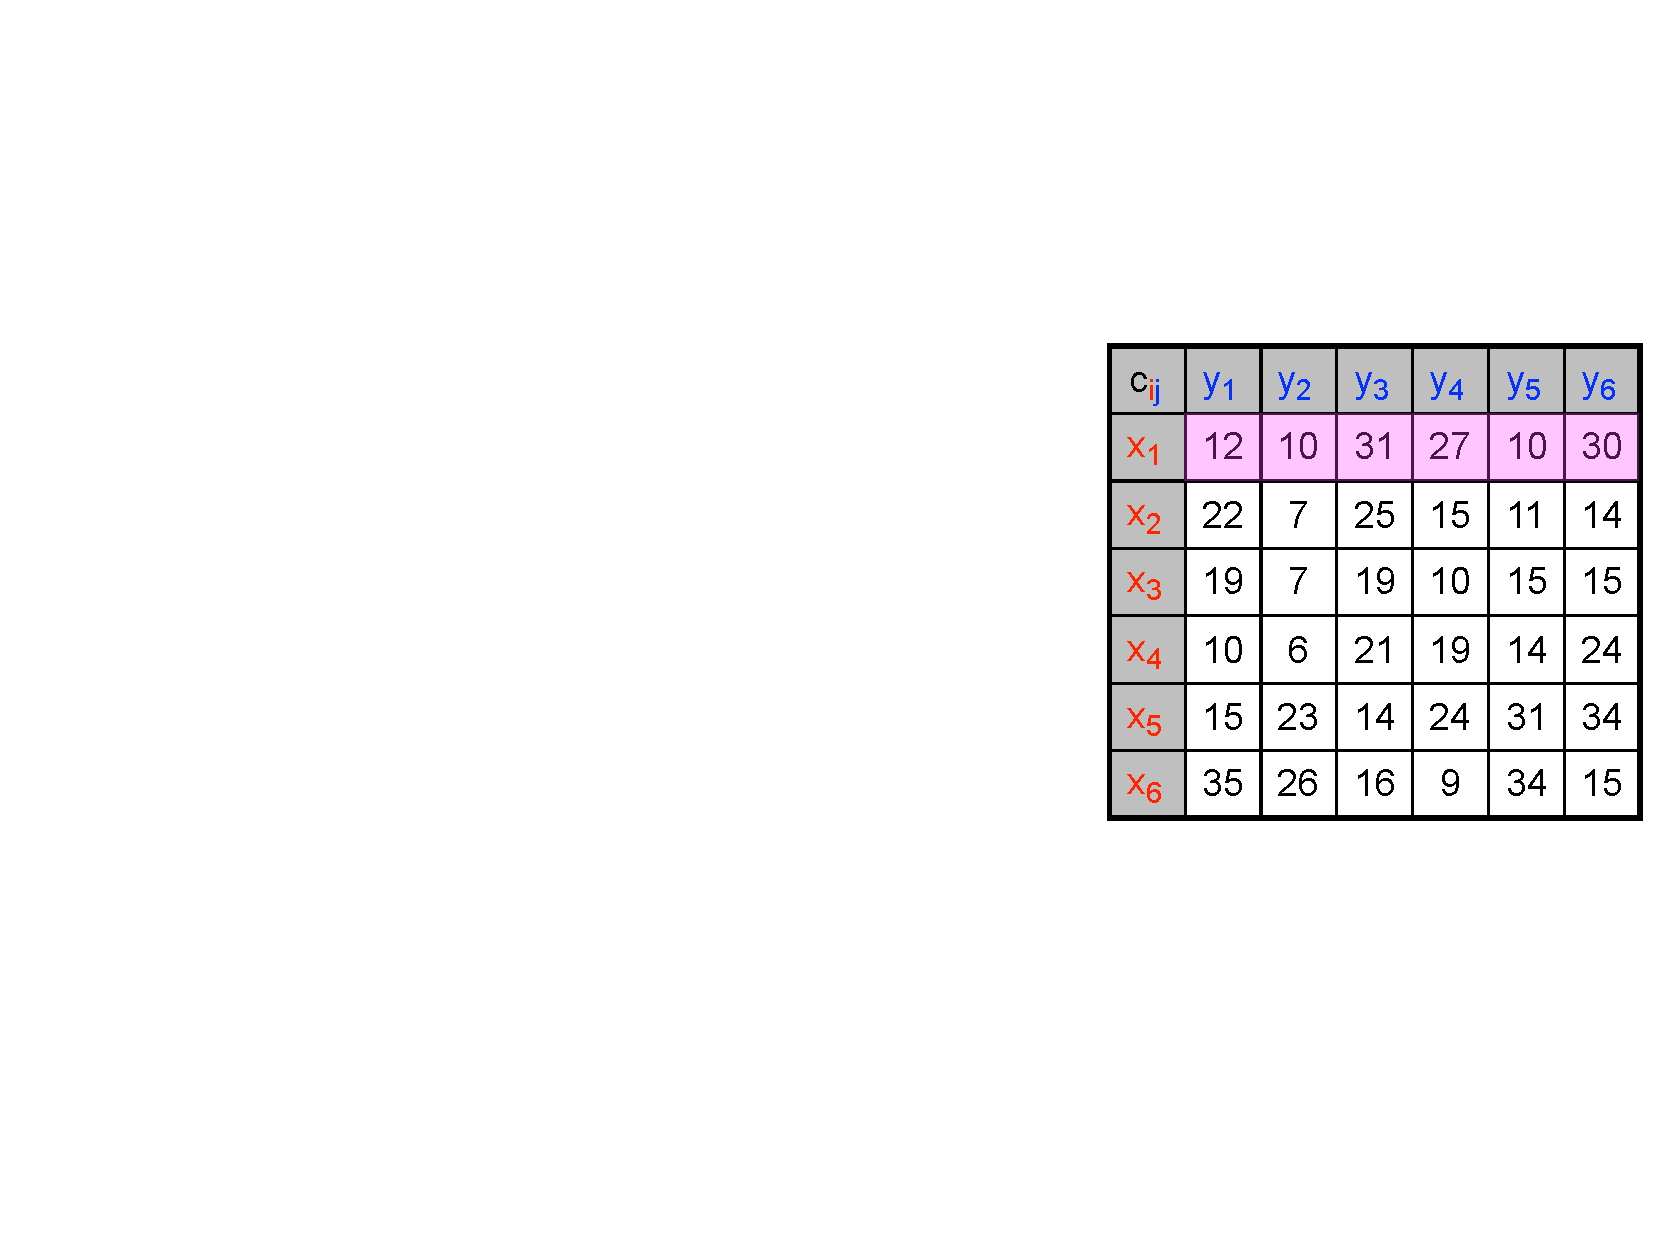
\includegraphics[width=.22\linewidth]{transport/cafe-paris/map-paris-0-couts} 
        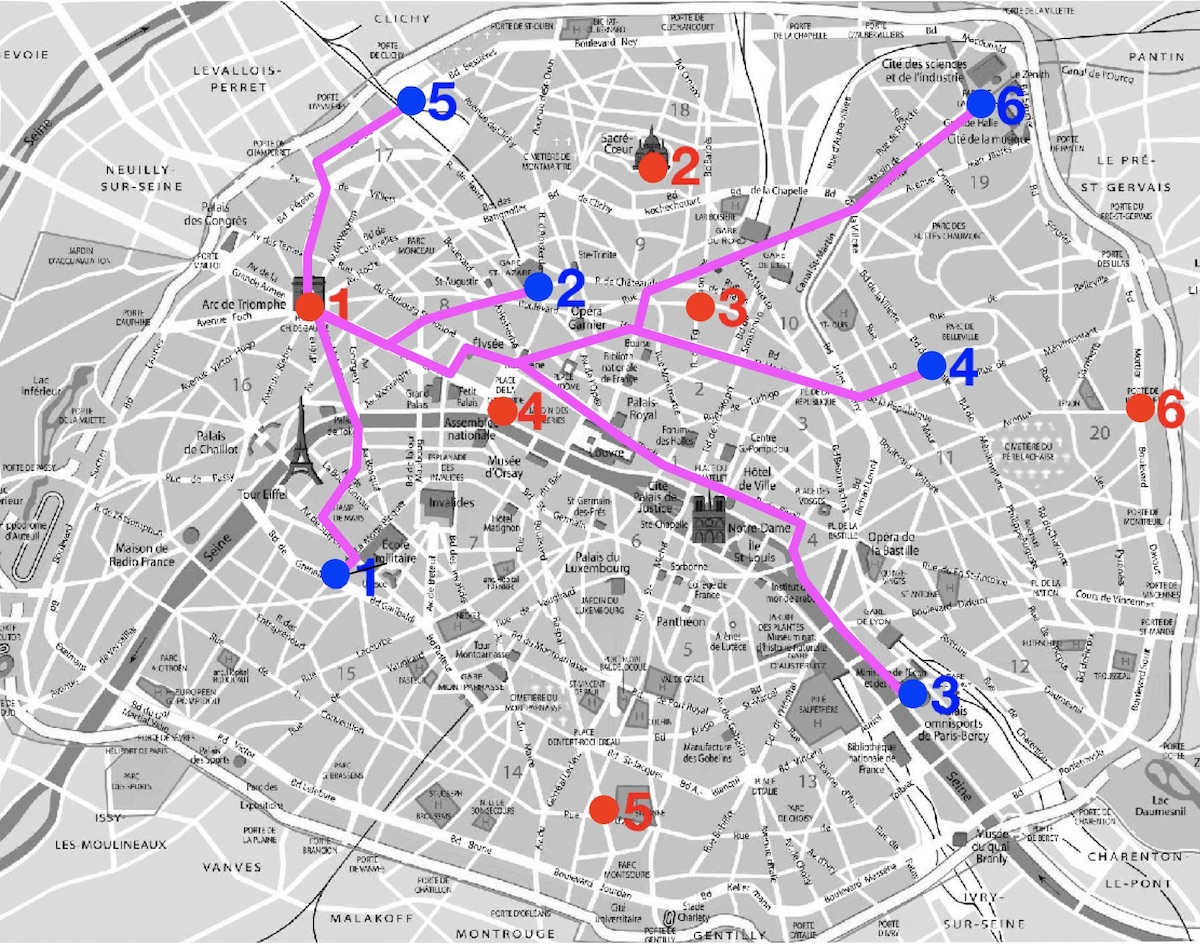
\includegraphics[width=.27\linewidth]{transport/cafe-paris/map-paris-0} 
        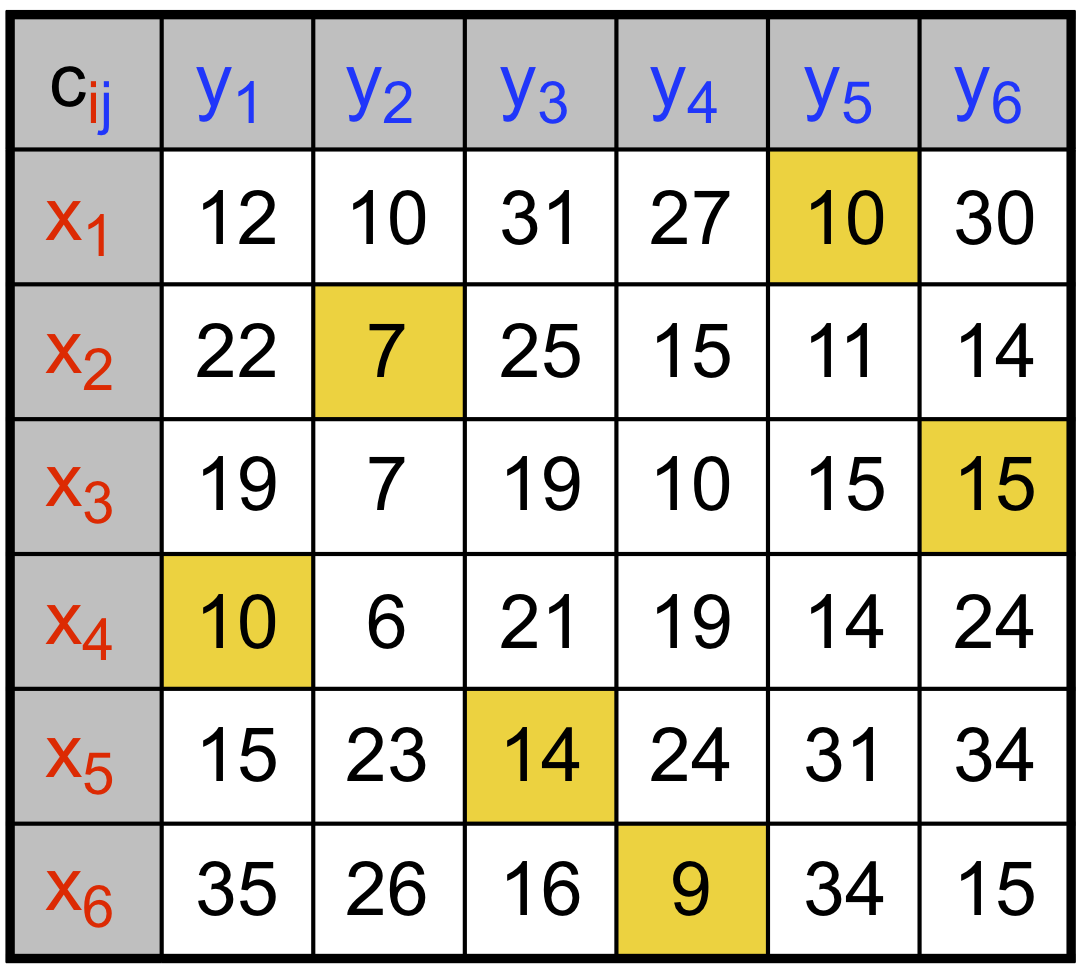
\includegraphics[width=.22\linewidth]{transport/cafe-paris/map-paris-1-couts} 
        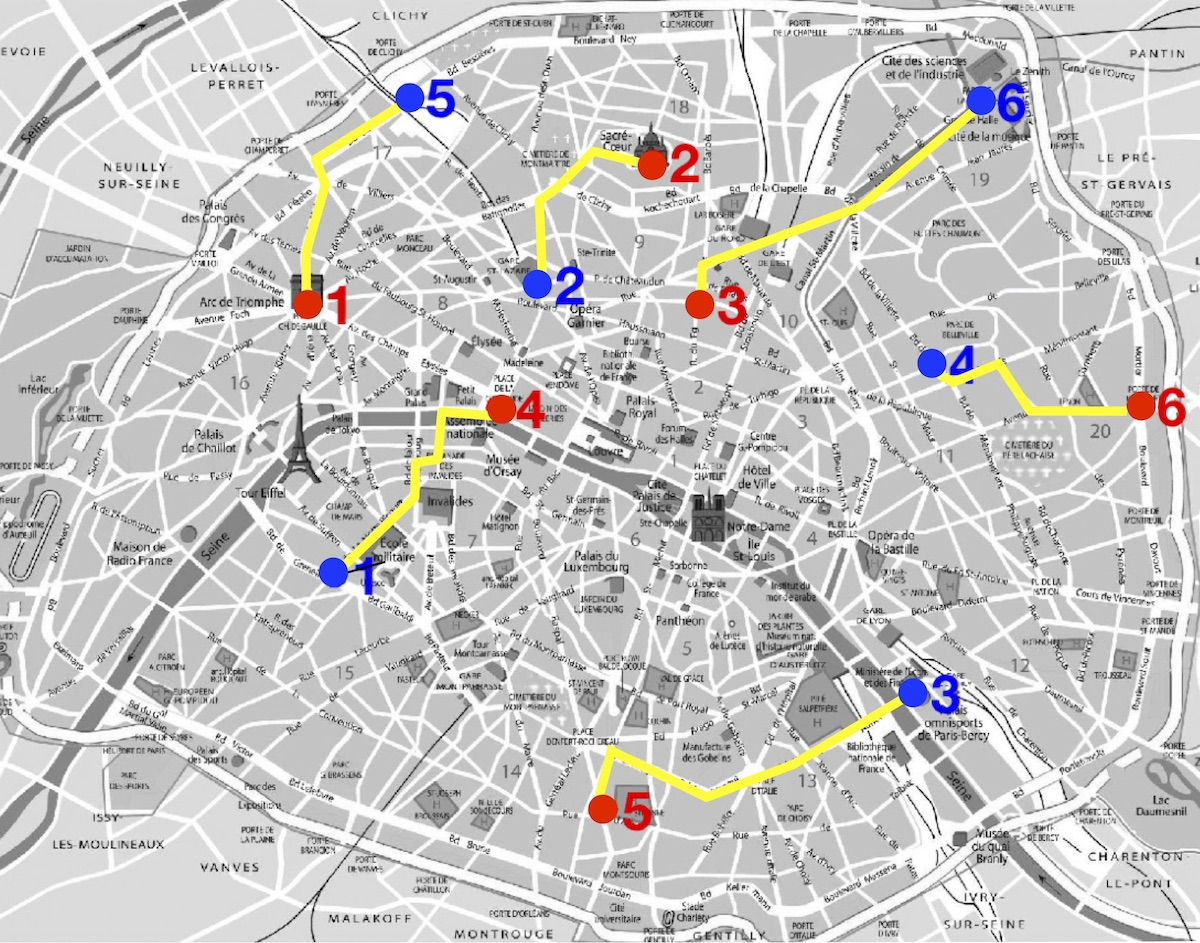
\includegraphics[width=.27\linewidth]{transport/cafe-paris/map-paris-1} 
    \end{tabular}
    \caption{\label{fig:image-cafe} Matrice de co�t et connexions associ�es. Gauche : une ligne de la matrice co�t. Droite : un exemple particulier de permutation. } 
\end{figure}

Afin de satisfaire la contrainte d'approvisionnement (que l'on appelle aussi la conservation de la masse), il faut que chaque boulangerie soit connect�e � un et un seul caf�. Comme il y a le m�me nombre de boulangeries que de caf�s, ceci implique que chaque caf� est �galement connect� � une et une seule boulangerie. On va noter 
\eq{    
    \si : \iC \in \{1,\ldots,6\} \longmapsto \jC \in \{1,\ldots,6\}
}
un tel choix de connexions. La figure~\ref{fig:image-cafe} illustre au centre et � droite l'exemple
\eql{\label{eq-bijection-exmp}
    \si(\Red{1})=\Blu{5}, \;
    \si(\Red{2})=\Blu{2}, \;
    \si(\Red{3})=\Blu{6}, \;
    \si(\Red{4})=\Blu{1}, \;
    \si(\Red{5})=\Blu{3}, \;
    \si(\Red{6})=\Blu{4}.
}  
La contrainte de conservation de masse signifie que $\si$ est une bijection de l'ensemble $\{1,\ldots,6\}$ dans lui-m�me. On dit aussi que $\si$ est une permutation. 

Le co�t de transport associ� � une telle bijection est la somme des co�ts $C_{\iC,\si(\iC)}$ s�lectionn�s par la permutation $\si$, c'est-�-dire 
\eql{\label{eq:cout}
    \text{Co�t}(\si) \eqdef 
        C_{\Red{1},\si(\Red{1})} + 
        C_{\Red{2},\si(\Red{2})} + 
        C_{\Red{3},\si(\Red{3})} + 
        C_{\Red{4},\si(\Red{4})} + 
        C_{\Red{5},\si(\Red{5})} + 
        C_{\Red{6},\si(\Red{6})}. 
}
Par exemple, pour la bijection~\eqref{eq-bijection-exmp} montr�e � la figure~\ref{fig:image-cafe}, on obtient comme co�t
\eq{
    C_{\Red{1},\Blu{5}} + 
    C_{\Red{2},\Blu{2}} + 
    C_{\Red{3},\Blu{6}} + 
    C_{\Red{4},\Blu{1}} + 
    C_{\Red{5},\Blu{3}} + 
    C_{\Red{6},\Blu{4}} = 
    10 + 7 + 15 + 10 + 14 + 9 = 65. 
}


Le probl�me de Monge consiste � chercher la permutation $\si$ qui a le co�t minimum, c'est-�-dire r�soudre le probl�me d'optimisation
\eql{\label{eq:monge}
    \umin{\si \in \Si_6} \text{Co�t}(\si), 
}
o� l'on a not� $\Si_6$ l'ensemble des permutations de l'ensemble $\{1,\ldots,6\}$.


\begin{figure}\centering
    \begin{tabular}{@{}c@{\hspace{1mm}}c@{\hspace{1mm}}c@{\hspace{1mm}}c@{}}
        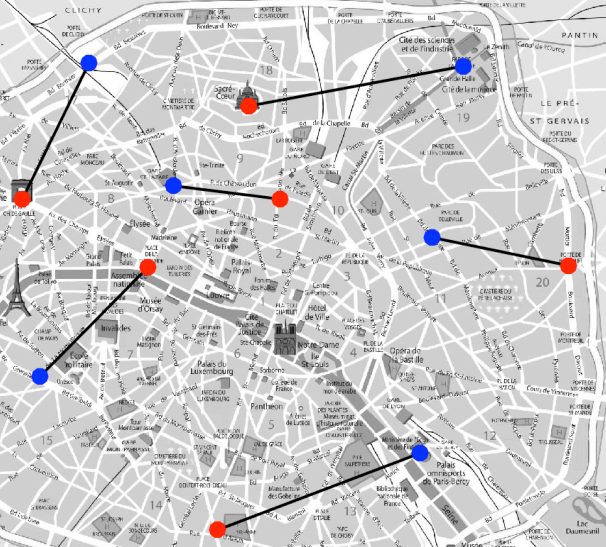
\includegraphics[width=.22\linewidth]{transport/cafe-paris/ordre-croissant-64}&
        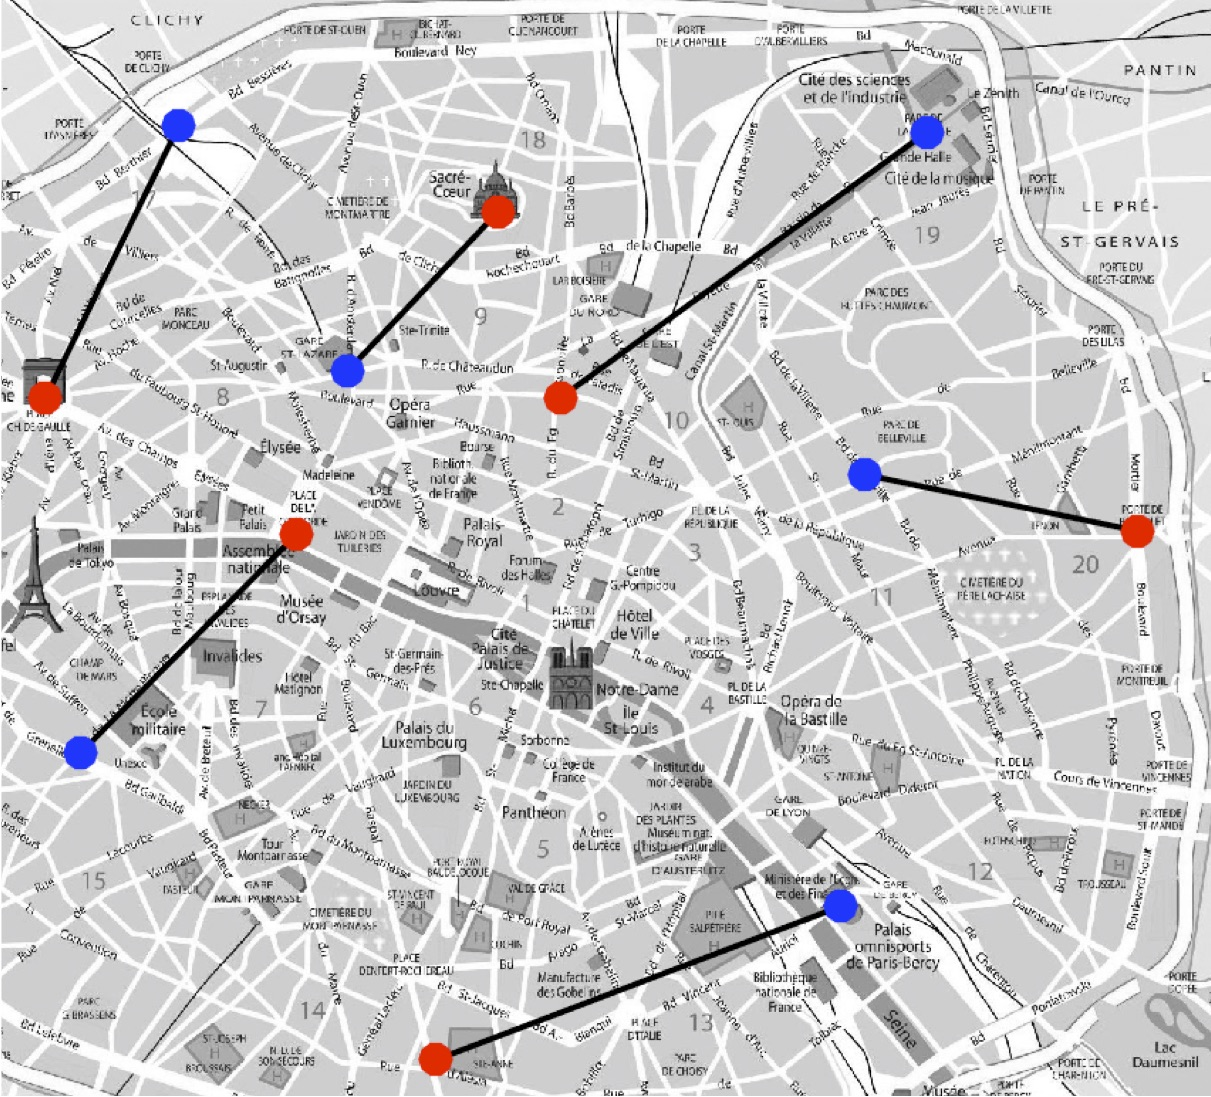
\includegraphics[width=.22\linewidth]{transport/cafe-paris/ordre-croissant-65}&
        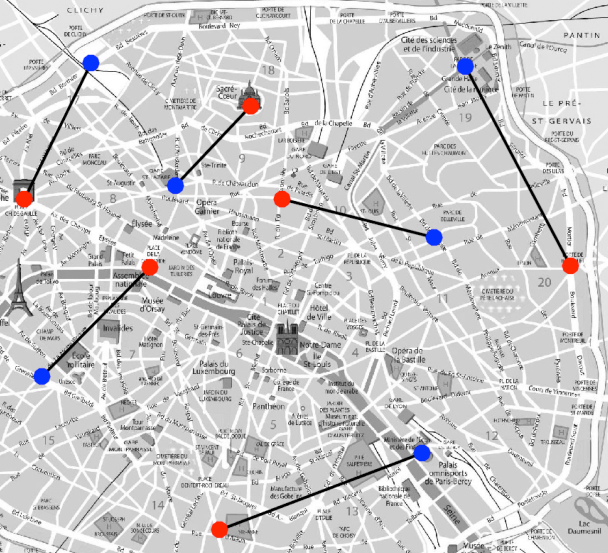
\includegraphics[width=.22\linewidth]{transport/cafe-paris/ordre-croissant-66}&
        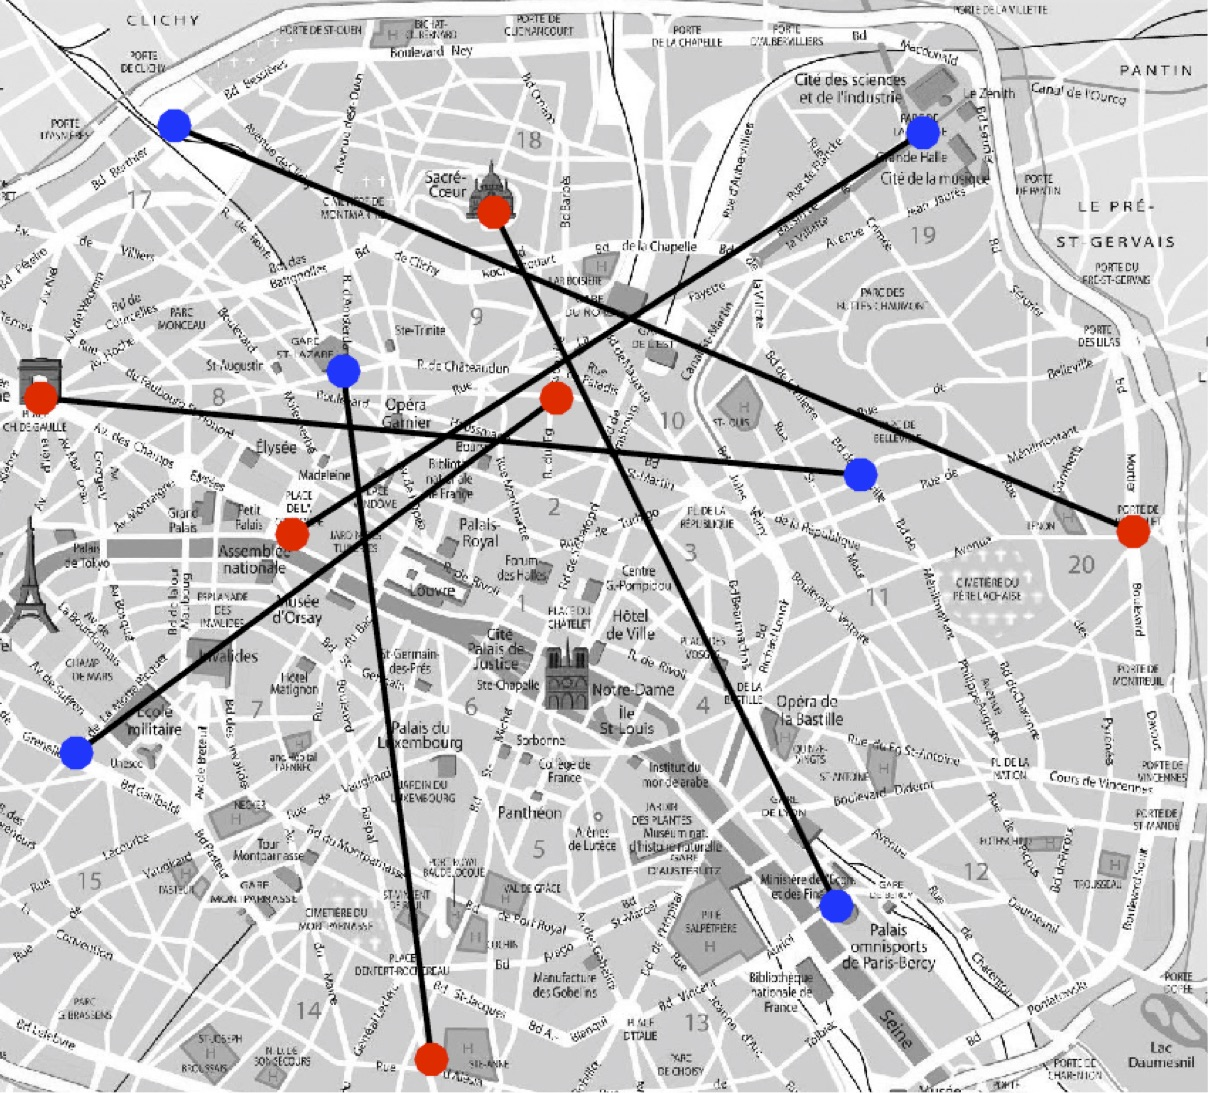
\includegraphics[width=.22\linewidth]{transport/cafe-paris/ordre-croissant-152}\\
        Co�t=64 &  
        Co�t=65 &  
        Co�t=66 &  
        Co�t=152
    \end{tabular}
    \caption{\label{fig:ordre-croissant} Exemples de permutations avec diff�rent co�ts. } 
\end{figure}

La figure~\ref{fig:ordre-croissant} montre que la permutation~\eqref{eq-bijection-exmp} n'est pas la meilleure : il existe par exemple une autre permutation qui a un co�t de 64. Mais est-ce la meilleure ? Il se trouve que oui, on peut en effet tester sur un ordinateur toutes les permutations de  $\{1,\ldots,6\}$ et calculer leur co�t. Combien y a-t-il de permutations au total ? Pour effectuer ce d�nombrement, on voit qu'il y a six choix d'affectation possible de $\Red{1}$ �  $\si(\Red{1}) \in \{\Blu{1,\ldots,6}\} $, puis cinq choix possibles pour affecter $\Red{2}$ � $\si(\Red{2}) \in  \{ \Blu{1,\ldots,6 } \}  - \{ \si(\Red{1}) \}$, et ainsi de suite. Le nombre total de possibilit�s est donc $6 \times 5 \times 4 \times 3 \times 2 \times 1 = 720$ que l'on note $6!$, \guill{factorielle 6}. Si on consid�re un nombre $n$ de boulangeries, alors le nombre de permutations � tester pour trouver la meilleure est $n! =n \times (n-1) \times \ldots \times 2 \times 1$. Ce nombre croit extr�mement vite avec $n$, par exemple $70! \approx 1,198 \times 10^{100}$, � comparer avec les $10^{11}$ neurones dans le cerveau et les $10^{79}$ atomes dans l'univers. Cette strat�gie de recherche exhaustive n'est donc possible que pour de toute petites valeurs de $n$. 


\begin{figure}\centering
    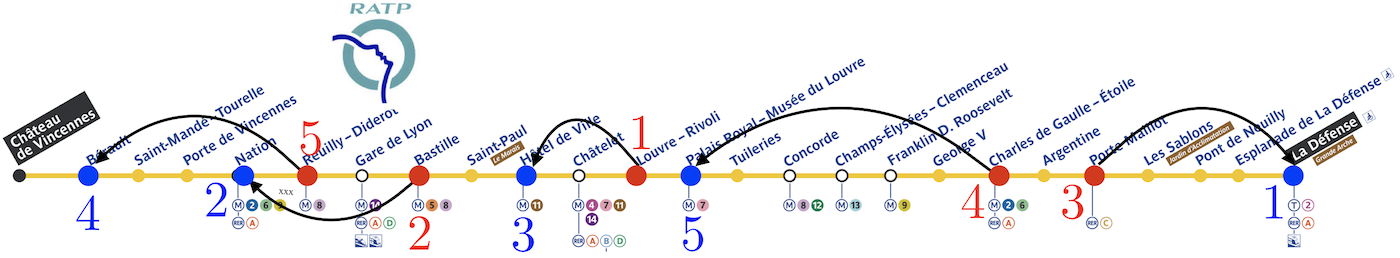
\includegraphics[width=.7\linewidth]{transport/metro/plan-metro}
    \caption{\label{fig:metro} Le transport optimal en 1D le long d'une ligne de m�tro. La bijection optimale est  
    $\si : (\Red{1,2,3,4,5}) \mapsto (\Blu{3,2,1,5,4})$. } 
\end{figure}

%%%%%%%%%%%%%%%%%%%%%%%%%%%%%%%
\myparagraph{En 1D et 2D}

La section~\ref{sec-kanto} explique comment des avanc�es math�matiques ont permis de d�velopper des techniques efficaces pour calculer un transport optimal $\si$ m�me pour de grandes valeurs de $n$. Mais il aura fallu attendre pr�s de 200 ans pour y arriver. Dans certains cas simples, on peut cependant calculer le transport optimal de fa�on simple. Le cas le plus �l�mentaire est lorsque les points � apparier sont le long d'un axe 1D, par exemple si les caf�s et les boulangeries sont situ�s le long d'une ligne de m�tro. Il faut �galement que le co�t $C_{\iC,\jC}$ soit la distance le long de cet axe (par exemple le temps de trajet en m�tro entre les stations). Dans ce cas, il suffit de classer les indices $\iC$ et $\jC$ par ordre croissant (donc de gauche � droite le long de la ligne de m�tro) et d'apparier le premier indice $\iC$ au premier indice $\jC$ ensemble, puis le deuxi�me indice, etc. Ce proc�d� est illustr� � la figure~\ref{fig:metro}.  Le temps de calcul n�cessaire pour calculer le transport optimal en m�tro est donc le temps n�cessaire pour classer les indices. L'algorithme le plus simple pour effectuer un classement est celui utilis� habituellement pour trier un jeu de $n$ cartes : il s'agit du tri par insertion, qui ins�re it�rativement chaque carte � sa place par rapport aux cartes d�j� class�es. Il effectue $n(n-1)/2$ comparaisons. Pour $n=70$, ceci n�cessite donc seulement 21415 operations, ce qui rend la m�thode utilisable, au contraire de la recherche exhaustive de toutes les $n!$ permutations.
% 
On dispose d'algorithmes encore plus rapides (par exemple le tri fusion), qui effectuent de l'ordre de $n \log(n)$ op�rations, et donc pour $n = 70$, de telles m�thodes n�cessitent moins de 1000 op�rations. 

Malheureusement, il n'est plus possible d'utiliser cette technique de classement dans des cas plus g�n�raux. Pour des points en dimension 2, si on prend comme co�t $C_{\iC,\si(\iC)}$ la distance euclidienne (la distance en vol d'oiseau) entre les points, alors Gaspard Monge a montr� dans son papier original (voir la figure~\ref{fig:ot2d}, � gauche) qu'un transport optimal ne peut par contenir de croisement. Par exemple, comme le montre la figure~\ref{fig:ot2d} (� droite), si l'on trace tous les segments entre les points $\iC \mapsto \jC = \si(\iC)$  que l'on relie par la bijection d�finie par $\si$, ceux-ci ne se croisent jamais. 

\begin{figure}\centering
    \begin{tabular}{@{}c@{\hspace{6mm}}c@{\hspace{3mm}}c@{}} % c@{\hspace{1mm}}
        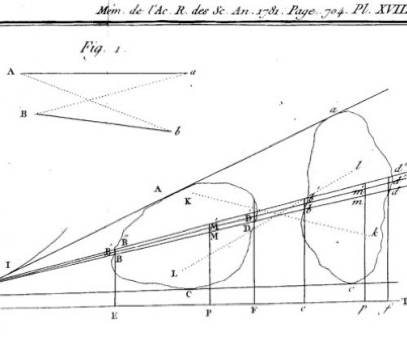
\includegraphics[width=.22\linewidth]{transport/monge-2d/article-monge}&
%        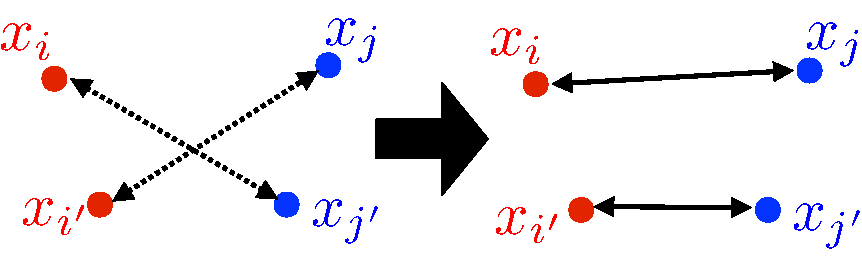
\includegraphics[width=.22\linewidth]{transport/monge-2d/decroisement}&
        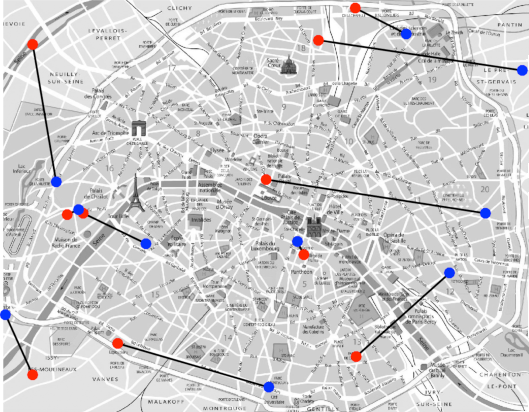
\includegraphics[width=.22\linewidth]{transport/monge-2d/example-10}&
        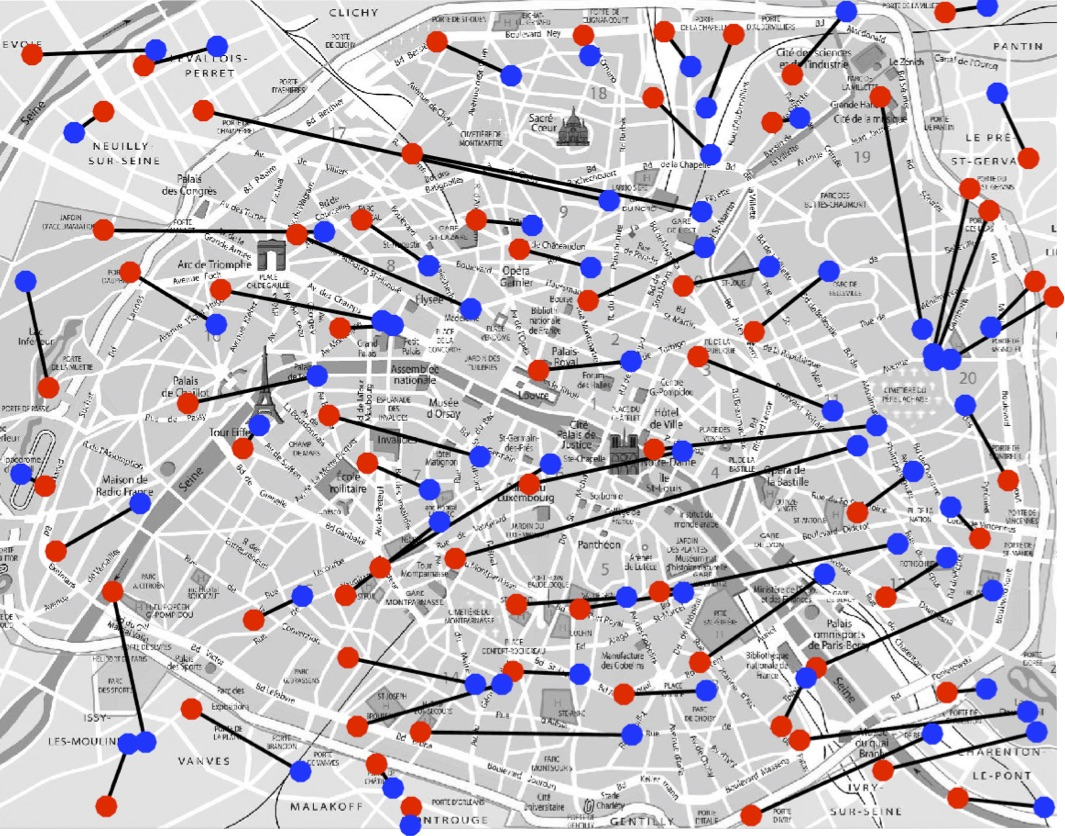
\includegraphics[width=.22\linewidth]{transport/monge-2d/example-70}
    \end{tabular}
    \caption{\label{fig:ot2d} Gauche: extrait de l'article de Monge~\cite{Monge1781}. Droite: le transport optimal en 2D pour un co�t euclidien.  } 
\end{figure}

Cette observation g�om�trique n'est cependant pas suffisante pour calculer un transport optimal en 2D : il existe en effet beaucoup de permutations $\si$ telles que les segments associ�s ne se croisent pas. 
%
Il va falloir analyser de fa�on plus fine la structure des permutations optimales afin de pouvoir les calculer de fa�on efficace. 
%
Nous allons maintenant voir comment Leonid Kantorovitch a reformul� le probl�me de Monge afin d'y parvenir. 


%%%%%%%%%%%%%%%%%%%%%%%%%%%%%%%%%%%%%%%%%%%%%%
\section{Le Transport Optimal de Kantorovitch}
\label{sec-kanto}

Leonid Kantorovitch est un math�maticien et un �conomiste sovi�tique qui a r�volutionn� la th�orie du transport optimal pendant les ann�es 40. Ses recherches sont issues de consid�rations pratiques qui l'ont occup� avant et apr�s la seconde guerre mondiale. Il y a jou� un r�le important pour assurer une distribution optimale des ressources, en particulier durant le si�ge de L�ningrad.
%
Il a par la m�me occasion particip� au d�veloppement de l'optimisation moderne, laquelle a eu un impact �norme dans de tr�s nombreux domaines appliqu�s. Il a ainsi obtenu en 1975 le prix Nobel d'�conomie, car les premi�res applications (mais certainement pas les seules !) de sa th�orie l'ont �t� dans ce domaine. 


%%%%%%%%%%%%%%%%%%%%%%%%%%%%%%%
\myparagraph{Le probl�me de Kantorovitch}

L'id�e centrale de Kantorovitch est de modifier le probl�me de Monge en rempla�ant l'ensemble des permutations par un ensemble plus grand mais plus simple. Tout d'abord on remarque que l'on peut repr�senter une permutation $\si$ � l'aide d'une matrice de permutation $P$ qui est une matrice binaire (remplie de 0 et de 1) de taille $n \times n$ telle que $P_{\iC,\jC} = 0$ sauf si $\jC=\si(\iC)$ auquel cas $P_{\iC,\si(\iC)} = 1$. Par exemple, pour $n=3$ points, les permutations 
$(\Red{1,2,3}) \mapsto (\Blu{1,2,3})$ (l'identit�), 
$(\Red{1,2,3}) \mapsto (\Blu{3,2,1})$ et
$(\Red{1,2,3}) \mapsto (\Blu{2,1,3})$ sont repr�sent�es par les matrices de taille $3 \times 3$
\eq{
	\begin{pmatrix} 1&0&0 \\ 0&1&0 \\ 0&0&1 \end{pmatrix}, \quad
	\begin{pmatrix} 0&0&1 \\ 0&1&0 \\ 1&0&0 \end{pmatrix} \qetq
	\begin{pmatrix} 0&1&0 \\ 1&0&0 \\ 0&0&1 \end{pmatrix}.
}
Dans la suite, on note $\Pp_n$ l'ensemble des $n!$ matrices de permutation de taille $n \times n$.

Comme la matrice est binaire, avec seulement $n$ �l�ments non-nuls �gaux � 1, on peut remplacer la somme de $n$ termes qui apparait dans $\text{Co�t}(\si)$ d�fini en~\eqref{eq:cout} par une somme sur l'ensemble des $n \times n$ indices $(\iC,\jC)$, c'est-�-dire que si $P$ est la matrice de permutation associ�e � $\si$, on a 
\eq{
	\text{Co�t}(\si) = \sum_{\iC=1}^n \sum_{\jC=1}^n P_{\iC,\jC} C_{\iC,\jC}.
}
On peut ainsi remplacer le probl�me de Monge~\eqref{eq:monge} par le probl�me �quivalent 
\eql{\label{eq:mongematrix}
    \umin{P \in \Pp_n}  \sum_{\iC=1}^n \sum_{\jC=1}^n P_{\iC,\jC} C_{\iC,\jC}.
}

Le g�nie de Kantorovitch a �t� de remarquer que l'on peut remplacer l'ensemble discret $\Pp_n$ (c'est-�-dire compos� d'un ensemble fini, mais tr�s grand, de $n!$ matrices) par un ensemble \guill{continu} (donc en particulier infini) mais plus simple. On remarque en effet que les matrices de permutation de $\Pp_n$ sont exactement les matrices qui ont un et un seul 1 le long de chaque ligne et de chaque colonne. Ceci peut aussi s'exprimer comme le fait qu'une matrice de permutation est une matrice binaire dont la somme de chaque ligne et de chaque colonne vaut 1, c'est-�-dire
\eq{
	\Pp_n = \enscond{ P \in \{0,1\}^{n \times n} }{ \foralls \iC, \sum_{\jC} P_{\iC,\jC}=1, \foralls \jC, \sum_{\iC} P_{\iC,\jC}=1  }.
}
Ce qui rend cet ensemble tr�s compliqu�, c'est la contrainte binaire, c'est-�-dire que ces matrices sont contraintes � �tre dans $\{0,1\}^{n \times n}$. Kantorovitch propose alors de \guill{relaxer} cette contrainte en supposant simplement que les entr�es de $P$ sont entre $0$ et $1$. Ceci d�finit un ensemble plus grand, l'ensemble des matrices bistochastiques 
\eql{\label{eq:bistoch}
	\Bb_n \eqdef \enscond{ P \in [0,1]^{n \times n} }{ \foralls \iC, \sum_{\jC} P_{\iC,\jC}=1, \foralls \jC, \sum_{\iC} P_{\iC,\jC}=1  }.
}
Le probl�me de Kantorovitch s'obtient en effectuant ce remplacement dans~\eqref{eq:mongematrix}, afin de r�soudre 
\eql{\label{eq:kantoassign}
    \umin{P \in \Bb_n} 
        \sum_{\iC=1}^n \sum_{\jC=1}^n P_{\iC,\jC} C_{\iC,\jC}.
}
L'immense avantage du probl�me de Kantorovitch~\eqref{eq:kantoassign} par rapport � celui de Monge~\eqref{eq:mongematrix} est que l'ensemble des matrices bistochastique est convexes, c'est-�-dire que si l'on consid�re deux matrices bistochastiques $P,Q \in \Bb_n$, alors leur moyenne $\frac{P+Q}{2} \in \Bb_n$ est encore bistochastique. Ceci n'est pas vrai pour les matrices de permutation, puisque la moyenne de deux matrices binaires $(P,Q)$ n'est pas binaire (sauf si bien s�r si $P=Q$). Cette convexit� est la clef pour le d�veloppement d'algorithmes efficaces. 
%
Cette nouvelle formulation a en effet pu b�n�ficier d'une deuxi�me r�volution initi�e par George Dantzig~\cite{Dantzig51}, qui, � la m�me �poque, a propos� l'algorithme du simplexe. Celui-ci permet de r�soudre efficacement une certaine classe de probl�mes d'optimisation convexe : les probl�mes de programmation lin�aire, dont~\eqref{eq:kantoassign} est un cas particulier. Dans le cas du probl�me de Kantorovitch, il existe en effet un algorithme du simplexe qui a une complexit� de l'ordre de $n^3$ op�rations, ce qui permet de faire des calculs pour de grands $n$, de l'ordre de plusieurs milliers. 


%%%%%%%%%%%%%%%%%%%%%%%%%%%%%%%
\myparagraph{L'�quivalence Monge--Kantorovitch}

L'ensemble des matrices bistochastiques est plus grand que celui des matrices de permutations, $\Pp_n \subset \Bb_n$, de sorte que l'on a l'in�galit� 
\eql{\label{eq:monge-vs-kanto}
    \umin{P \in \Bb_n} 
        \sum_{\iC=1}^n \sum_{\jC=1}^n P_{\iC,\jC} C_{\iC,\jC}
     \leq 
    \umin{P \in \Pp_n} 
        \sum_{\iC=1}^n \sum_{\jC=1}^n P_{\iC,\jC} C_{\iC,\jC}
}
entre les probl�mes de Kantorovitch et de Monge. Mais de fa�on � premi�re vue surprenante, un th�or�me fondamental d� � George Birkhoff et � John von Neumann~\cite{birkhoff,von1953certain} assure qu'en fait il y a �galit� entre les valeurs de ces deux minimisations. En effet, ce th�or�me montre qu'il existe toujours une matrice solution du probl�me de Kantorovitch qui est une matrice de permutation, de sorte qu'elle est aussi solution du probl�me de Monge. Attention cependant, en g�n�ral il n'y a pas unicit� des solutions de ces probl�mes : il peut exister une matrice bistochastique solution du probl�me de Kantorovitch qui n'est pas une permutation. 
%
La conjonction de deux avanc�es spectaculaires, dues � Kantorovitch et � Dantzig, a permis de rendre le transport optimal applicable � des probl�mes de grande taille, puisque l'algorithme du simplexe permet de r�soudre en pratique ces probl�mes. 

%%%%%%%%%%%%%%%%%%%%%%%%%%%%%%%
\myparagraph{Le cas pond�r�}

Outre son int�r�t pratique, la formulation de Kantorovitch a aussi permis de g�n�raliser le probl�me initial de Monge, en donnant le bon cadre pour le formaliser et l'�tudier math�matiquement. En effet, le probl�me de Monge est tr�s limit�. Que se passe-t-il par exemple si il n'y pas le m�me nombre $n$ de caf�s et $m$ de boulangeries ? Le probl�me initial~\eqref{eq:monge} n'a pas de solution, car on ne peut pas mettre en bijection deux ensembles de tailles diff�rentes. Le bon concept n'est pas le nombre de boulangeries et de caf�s, mais plut�t les distributions $(\Red{a_1,\ldots,a_n})$ de production (associ�es au boulangeries) et les distributions $(\Blu{b_1,\ldots,b_m})$ de consommation des caf�s.  Dans le cas initialement consid�r�, o� $n=m$, toutes les quantit�s $\Red{a_i}$ et $\Blu{b_j}$ sont �gales � 1. Mais dans de nombreux cas concrets, ces quantit�s sont quelconques. Ces quantit�s doivent �tre positives, et v�rifier 
\eq{
	\Red{a_1+\cdots+a_n} = \Blu{b_1 + \cdots + b_m}, 
}
de sorte qu'il y ait autant de production que de consommation. La construction de Kantorovitch s'adapte naturellement � ce cas de distributions g�n�rales, en rempla�ant les matrices bistochastique~\eqref{eq:bistoch} par des matrices de \guill{couplage} qui satisfont la contrainte de conservation de la masse 
\eq{
	\Bb(\aC,\bC) \eqdef \enscond{ P \in [0,1]^{n \times m} }{ \foralls \iC, \sum_{\jC} P_{\iC,\jC}=\Red{a_i}, \foralls \jC, \sum_{\iC} P_{\iC,\jC}= \Blu{b_j}  }.
}
Dans le cas initial o� $n=m$ et $\Red{a_i}=\Blu{b_j}=1$, alors $\Bb(\aC,\bC) = \Bb_n$ et l'on retrouve des matrices bistochastiques. Dans le cas g�n�ral, � chaque fois qu'une entr�e $P_{\iC,\jC}$ est non-nulle, ceci signifie que l'on transfert de la \guill{masse} (ici une certaine quantit� de croissants) entre $\iC$ et $\jC$. Comme le montre la figure~\ref{fig:coupling-visu}, on peut visualiser de diff�rentes fa�ons une telle matrice $P$ couplant deux distributions $(\aC,\bC)$.
%
Contrairement au cas des matrices bistochastiques, pour lequel il y a toujours une solution qui est une permutation, ici un couplage optimal $\Bb(\aC,\bC)$ peut avoir plus d'une seule entr�e non-nulle $P_{\iC,\jC}$ le long d'une ligne index�e par $\iC$ (voir la figure~\ref{fig:coupling-visu}). Ceci signifie que cette boulangerie $\iC$ est connect�e � plusieurs caf�s, de sorte que sa production est alors s�par�e en plusieurs lots de croissants distribu�s, tout en satisfaisant la contrainte de conservation de la masse $\sum_{\jC} P_{\iC,\jC}=\Red{a_i}$.

\begin{figure}\centering
    \begin{tabular}{@{}c@{\hspace{1mm}}c@{\hspace{1mm}}c@{\hspace{1mm}}c@{}}
        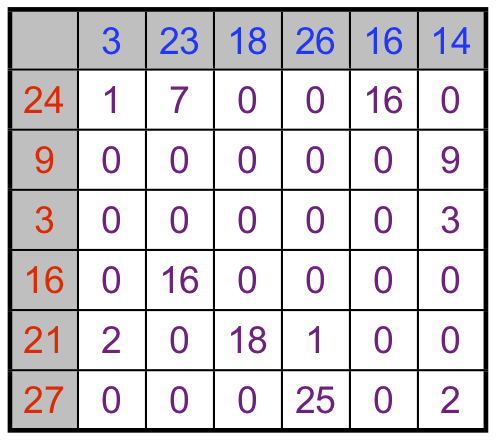
\includegraphics[width=.22\linewidth]{transport/kantorovitch/coupling-array}&
        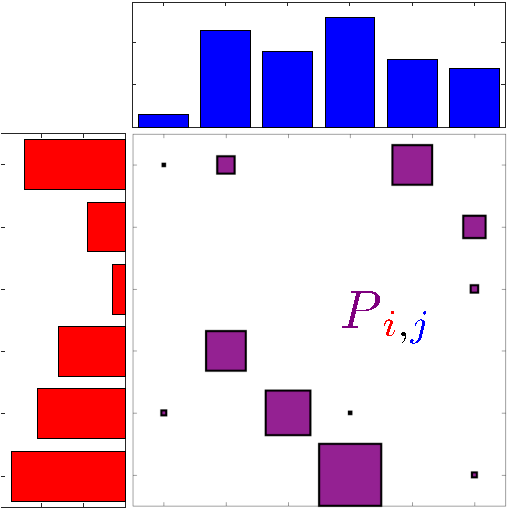
\includegraphics[width=.22\linewidth]{transport/kantorovitch/coupling-squares}&
        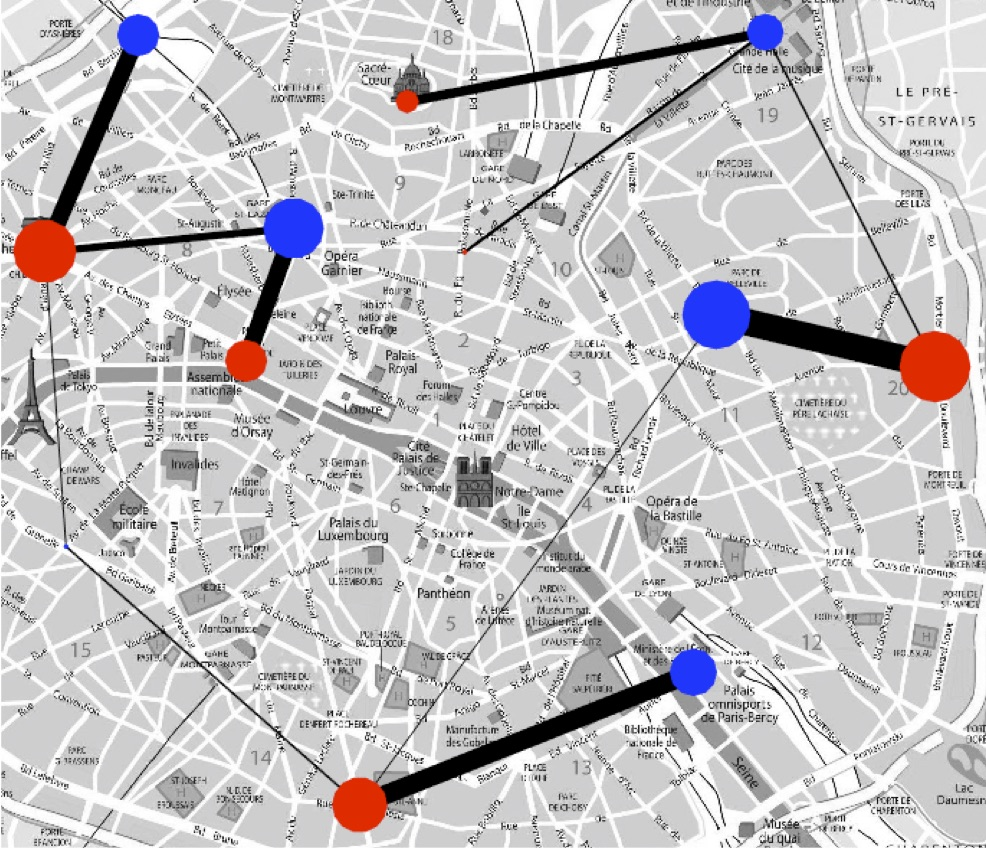
\includegraphics[width=.22\linewidth]{transport/kantorovitch/coupling-map}&
        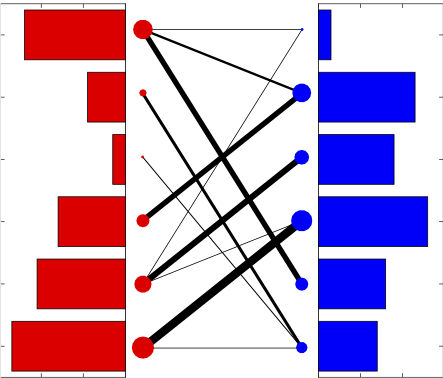
\includegraphics[width=.22\linewidth]{transport/kantorovitch/coupling-bipartite} \\
        (a) matrice & (b) histogrammes & (c) segments & (d) graphe biparti
    \end{tabular}
    \caption{\label{fig:coupling-visu} Diff�rentes fa�ons de repr�senter une matrice de couplage $P \in \Bb(\aC,\bC)$:
    	(a) un tableau de nombres dont les lignes et colonnes ont des sommes prescrites ; 
		(b) un histogramme bidimensionnel dont la taille de carr� est propositionnelle � $P_{\iC,\jC}$ ; 
		(c) un ensemble de segments dont la largeur est proportionnelle est  $P_{\iC,\jC}$. 
		(d) un graphe biparti, c'est-�-dire avec deux ensembles de sommets tels que les arr�tes soient seulement entre ces deux ensembles.   } 
\end{figure}


Le probl�me de Kantorovitch qui g�n�ralise~\eqref{eq:kantoassign} s'�crit alors
\eql{\label{eq-kanto-gen}
    \umin{P \in \Bb(\aC,\bC)} 
        \sum_{\iC=1}^n \sum_{\jC=1}^m P_{\iC,\jC} C_{\iC,\jC}
}
ce qui signifie que l'on doit payer un co�t  $C_{\iC,\jC}$ � chaque fois que l'on transfert une unit� de masse entre $\iC$ et $\jC$. Tout comme le probl�me original~\eqref{eq:kantoassign}, on peut le r�soudre de fa�on efficace avec l'algorithme du simplexe.  La figure~\ref{fig:coupling-visu} montre un exemple de couplage optimal. 



%%%%%%%%%%%%%%%%%%%%%%%%%%%%%%%%%%%%%%%%%%%%%%
\section{Les applications}

Bien que les motivations initiales de Monge et Kantorovitch �taient �t� respectivement militaires et �conomiques, le transport optimal a trouv� d'innombrables applications, � la fois th�oriques mais aussi plus concr�tes. Sur le plan math�matique, on peut consid�rer des distributions \guill{continues} de masses, en quelque sorte la limite quand le nombre de point $n$ tend vers l'infini. Ceci permet de d�finir le probl�me de transport entre des mesures de probabilit�s quelconques. Ce point de vue th�orique est extr�mement fructueux, et c'est le math�maticien fran�ais Yann Brenier qui a le premier montr� l'�quivalence dans le cadre continu des formulations de Monge et de Kantorotich~\cite{Brenier91}. Ces travaux pionniers ont montr� la connexion entre le probl�me de transport et les �quations aux d�riv�es partielles, et ont d�bouch�, entre autres, sur les m�dailles Fields de C�dric Villani (2010) et Alessio Figalli (2018). 

\begin{figure}\centering
\begin{tabular}{@{}c@{\hspace{1mm}}c@{\hspace{1mm}}c@{}}
    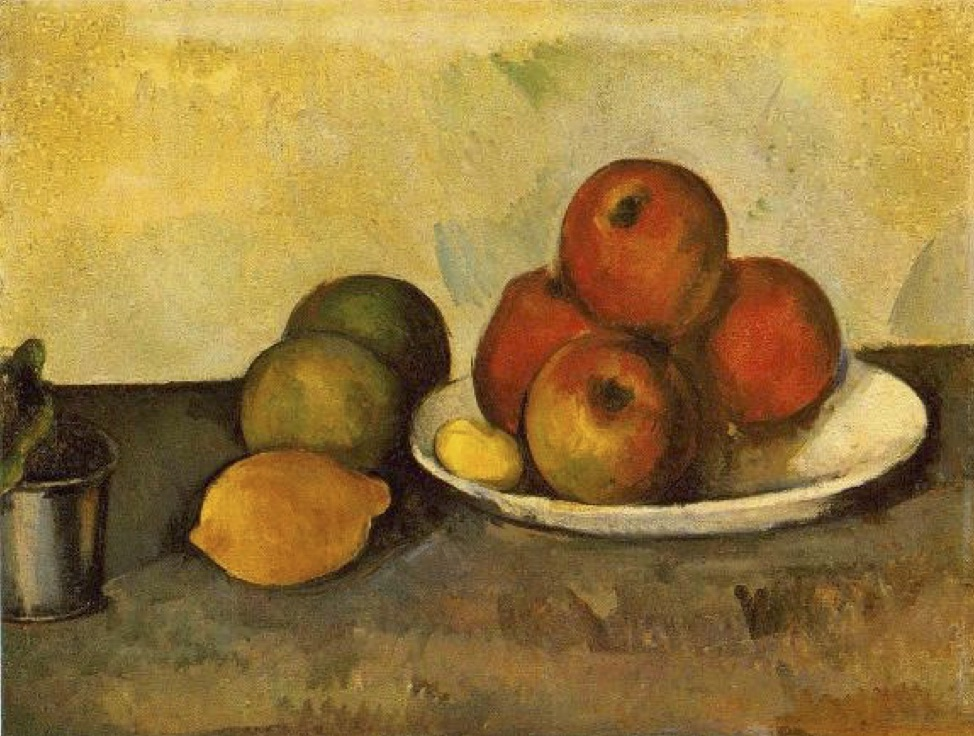
\includegraphics[width=.24\linewidth]{transport/applis/painting-2} &
    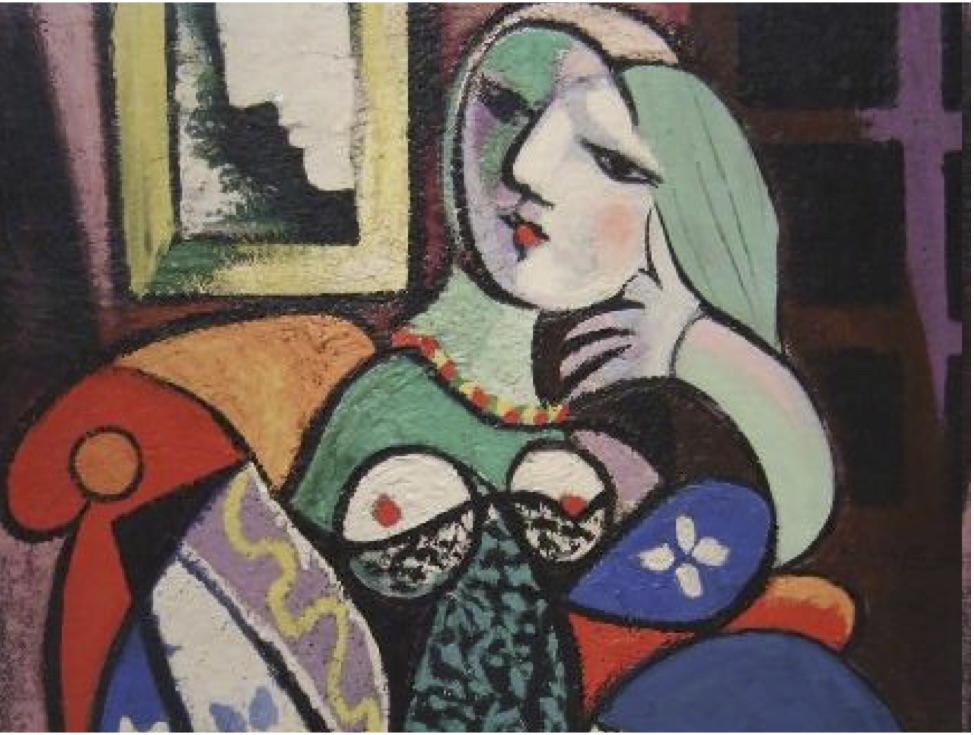
\includegraphics[width=.24\linewidth]{transport/applis/painting-1} &
    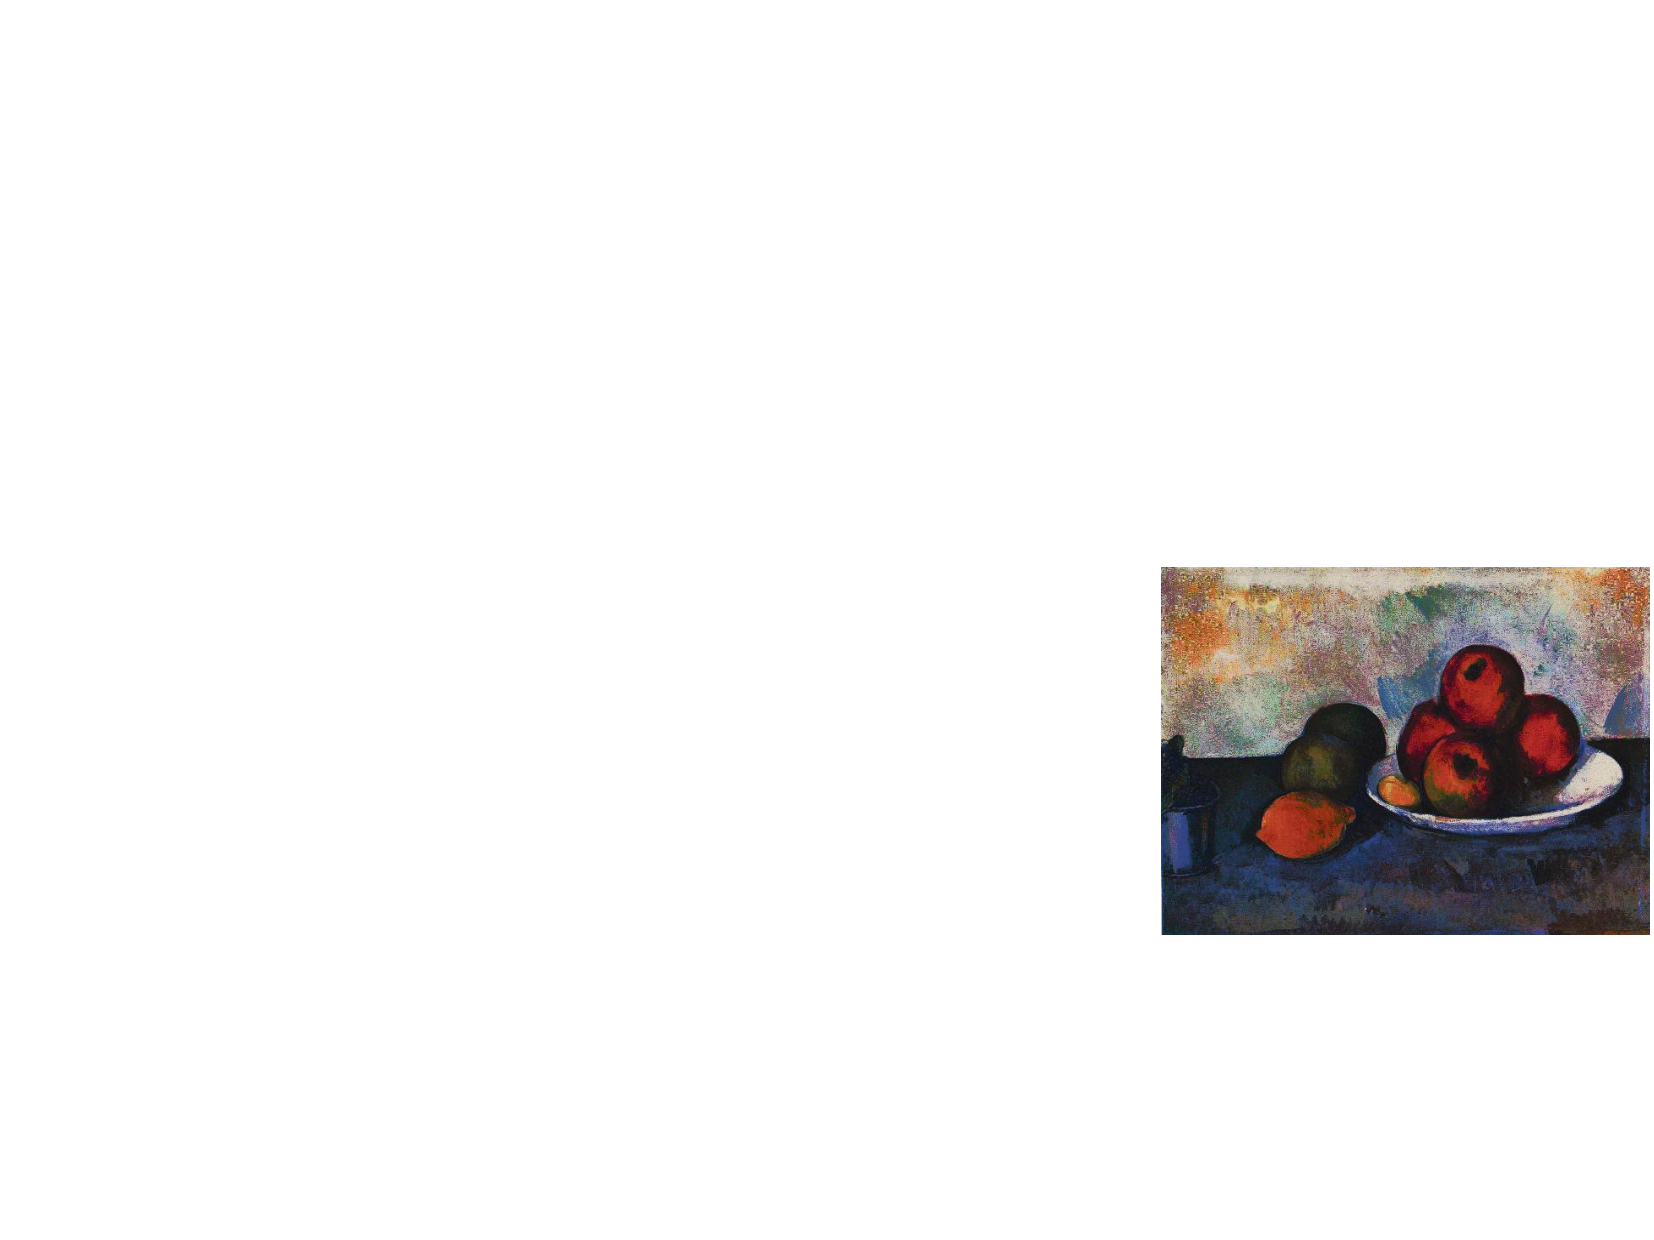
\includegraphics[width=.24\linewidth]{transport/applis/painting-2-equalized} \\
    Image $(\Red{x_i})_{\iC=1}^n$ & Image $(\Blu{y_j})_{\jC=1}^n$ & Image  $(y_{\si(\iC)})_{\iC=1}^n$ \\
    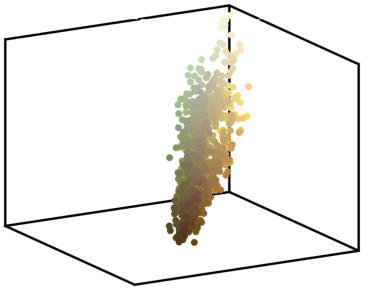
\includegraphics[width=.24\linewidth]{transport/applis/painting-2-histo}&
    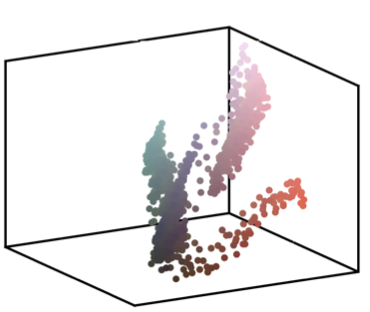
\includegraphics[width=.24\linewidth]{transport/applis/painting-1-histo}&
    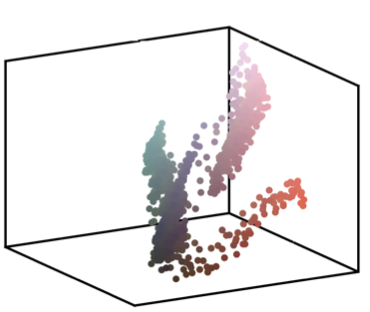
\includegraphics[width=.24\linewidth]{transport/applis/painting-1-histo}
\end{tabular}
\caption{\label{fig:image-eq} Exemple de transfert de palettes de couleurs � l'aide du transport optimal. 
	Haut: les pixels sont sur la grille d'affichage pour former une image couleur. 	
	Bas: les pixels sont plac�s � leurs positions dans $\RR^3$ pour former un nuage de points. }
\end{figure}

Le transport optimal est depuis peu au c\oe{}ur de probl�matiques plus appliqu�es en sciences des donn�es, en particulier pour r�soudre des probl�mes en traitement d'image et en apprentissage machine. 
%
La premi�re id�e, la plus imm�diate, est d'utiliser la bijection $\si$ afin de transformer des donn�es, par exemple des images. Dans ce cas, on consid�re les pixels $(\Red{x_i})_{\iC=1}^n$ et $(\Blu{y_j})_{\jC=1}^n$ de deux images couleur. Chaque pixel $\Red{x_i}, \Blu{y_j} \in \RR^3$ est un vecteur de dimension 3, qui repr�sente les intensit�s de chacune des trois couleurs �l�mentaires, rouge, vert et bleu. Afin de changer les couleurs de la premi�re image, et lui imposer la palette de la deuxi�me image, on calcule le transport $\si$ pour la matrice de co�t $C_{\iC} = \norm{\Red{x_i} - \Blu{y_j}}^2$ (c'est-�-dire le carr� de la norme euclidienne dans $\RR^3$), c'est-�-dire le carr� de la distance euclidienne entre les pixels. L'image avec les couleurs modifi�es est $(y_{\si(\iC)})_{\iC=1}^n$, c'est � dire que l'on remplace dans la premi�re image le pixel $\Red{x_i}$ par le pixel $y_{\si(\iC)}$. Cette image ressemble � la premi�re, mais a la palette de couleurs de la deuxi�me image.
%
La figure~\ref{fig:image-eq} illustre ce proc�d� pour imposer la palette de couleurs de Picasso � un tableau de C�zanne. 

On peut �galement utiliser le transport optimal pour des probl�mes plus difficiles, en n'utilisant que de fa�on indirecte la bijection $\si$ ou bien la matrice de couplage optimal $P \in \Bb(\aC,\bC)$. L'id�e centrale est que la quantit� associ�e � un couplage optimal $P$ solution de~\eqref{eq-kanto-gen}
\eq{
	W(\aC,\bC) \eqdef \sum_{i,j} P_{\iC,\jC} C_{\iC,\jC}
}
d�finit en quelque sorte l'effort n�cessaire pour d�placer la masse de la distribution $\aC$ vers la distribution $\bC$. Elle permet donc de quantifier combien ces deux distributions sont \guill{proches}. Par exemple, si $C_{\iC} = \norm{\Red{x_i} - \Blu{y_j}}^p$ est associ� � la distance euclidienne entre des points, pour $p \geq 1$, alors la quantit� $W(\aC,\bC)^{1/p}$ est une distance entre les distributions, en particulier elle v�rifie $W(\aC,\bC)=0$ si et seulement si $\aC=\bC$, et elle v�rifie l'in�galit� triangulaire. Ces propri�t�s sont tr�s importantes pour permettre d'appliquer le transport � des probl�mes pratiques.


\begin{figure}\centering
        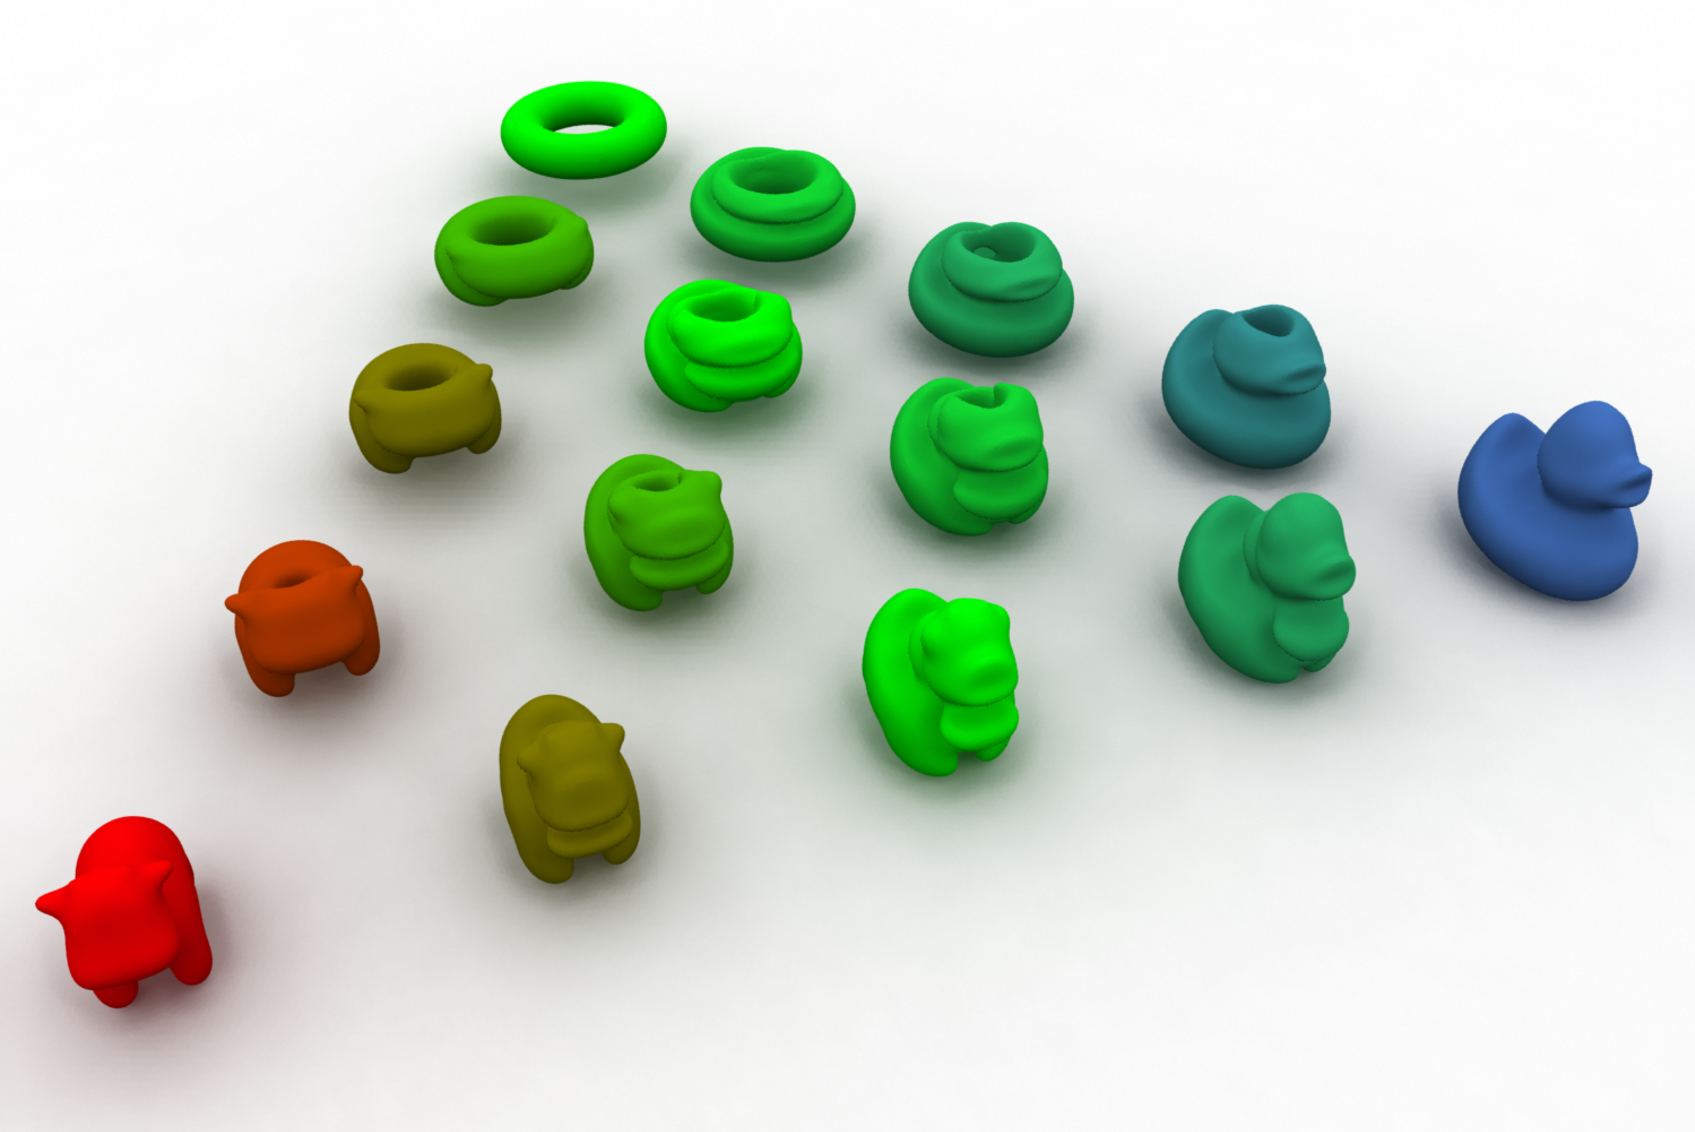
\includegraphics[width=.6\linewidth]{transport/applis/shapes-3d}
    \caption{\label{fig:barycenters} Exemple d'interpolation barycentrique entre des formes 3D, obtenu en minimisant~\eqref{eq-bary}.  }
\end{figure}

Un exemple typique d'application consiste � calculer des barycentres entre des distributions~\cite{agueh2011barycenters}. La figure~\ref{fig:barycenters} montre un exemple o� l'on consid�re trois distributions $a^1,a^2,a^3$ (montr�es aux trois sommets du triangles) qui sont des distributions uniformes de masse � l'int�rieur de formes 3D (c'est-�-dire que la masse $a^1_i$ associ�e � chaque point est 0 � l'ext�rieur de la premi�re forme et constante � l'int�rieur). On calcule un barycentre pond�r� $b$ de ces trois distributions en minimisant une somme pond�r�e de distances de transport optimal
\eql{\label{eq-bary}
	\umin{b} \la_1 W(a^1,b) + \la_1 W(a^2,b) + \la_1 W(a^3,b).
}
En modifiant les poids $(\la^1,\la^2,\la^3)$, qui sont positifs et tels que $\la^1+\la^2+\la^3=1$, on modifie la forme obtenue en se d�pla�ant � l'int�rieur d'un triangle de transport optimal. 
%
On peut utiliser cette distance $W$ pour bien d'autres applications o� l'on doit comparer des distributions de probabilit�. C'est le cas en apprentissage machine, par exemple pour comparer des textes � l'aide des distributions des mots qui les composent. La figure~\ref{fig:bagwords} illustre les histogrammes d'apparition des mots pour deux textes, o� la taille des lettres du mot $\iC$ est proportionnelle � la masse $\aC_\iC$. Une question difficile dans ce cas est de savoir quelle matrice de co�t $C_{\iC,\jC}$ utiliser entre deux mots $(\iC,\jC)$. Il s'agit d'un travail de linguistique (caract�riser la proximit� s�mantique entre des mots du langages), que l'on peut chercher � r�soudre en m�me temps que le transport optimal~\cite{huang2016supervised}. 

\begin{figure}\centering
    
\includegraphics[width=.35\linewidth]{transport/applis/bag-word-1}
    \qquad
    
\includegraphics[width=.35\linewidth]{transport/applis/bag-word-2}
\caption{\label{fig:bagwords} Exemples d'histogrammes de distributions des mots dans deux textes diff�rents (seuls les mots les plus fr�quents sont montr�s).  }
\end{figure}


%%%%%%%%%%%%%%%%%%%%%%%%%%%%%%%%%%%%%%%%%%%%%%
\section*{Conclusions}

Le transport optimal a connu de nombreuses r�volutions. Sous l'impulsion de math�maticiens tels que Monge, Kantorovitch, Dantzig et Brenier, il est progressivement devenu un outil th�orique et num�rique fondamental. 
%
Il est maintenant au c\oe{}ur de questions importantes en science des donn�es pour mod�liser, r�soudre num�riquement et analyser th�oriquement les probl�mes de l'apprentissage machine. Les opportunit�s pour d�velopper de nouvelles th�ories et des algorithmes performants sont immenses. 
%
Pour plus d'informations sur les aspects th�oriques du transport optimal, on pourra consulter les livres~\cite{Villani03,SantambrogioBook}. Les aspects num�riques et applicatifs sont couverts dans le livre~\cite{PeyreCuturi}.


%%%%%%%%%%%%%%%%%%%%%%%%%%%%%%%%%%%%%%%%%%%%%%
\section*{Remerciements}

Je tiens � remercier Vincent Beck, Gwenn Guichaoua et Marie-No�lle Peyr� pour leurs relectures attentives. 


